% PP-Article.tex for AEA last revised 22 June 2011
\documentclass[10pt, twocolumn, a4paper]{article}

%%%%%% NOTE FROM OVERLEAF: The mathtime package is no longer publicly available nor distributed. We recommend using a different font package e.g. mathptmx if you'd like to use a Times font.
\usepackage{mathptmx}
\usepackage{amsmath}
\usepackage[dutch]{babel}
\usepackage{subcaption}
\usepackage[width=.8\textwidth]{caption}
\usepackage{float}
\usepackage{booktabs}
\usepackage{multicol}
\usepackage{minted}
% If you have trouble with the mathtime package please see our technical support 
% document at: http://www.aeaweb.org/templates/technical_support.pdf
% You may remove the mathtime package if you can't get it working but your page
% count may be inaccurate as a result.
% \usepackage[cmbold]{mathtime}
\usepackage{xargs}                      % Use more than one optional parameter in a new commands
\usepackage[pdftex,dvipsnames]{xcolor}  % Coloured text etc.
% 
\usepackage{pdfpages}
\usepackage[colorinlistoftodos,prependcaption,textsize=tiny]{todonotes}
\newcommandx{\unsure}[2][1=]{\todo[linecolor=red,backgroundcolor=red!25,bordercolor=red,#1]{#2}}
\setlength{\marginparwidth}{2cm}
% Note: you may use either harvard or natbib (but not both) to provide a wider
% variety of citation commands than latex supports natively. See below.

% Uncomment the next line to use the natbib package with bibtex 
%\usepackage{natbib}
\usepackage{titlesec}

\titlespacing*\section{0pt}{12pt plus 4pt minus 2pt}{0pt plus 2pt minus 2pt}
\titlespacing*\subsection{0pt}{12pt plus 4pt minus 2pt}{0pt plus 2pt minus 2pt}
\titlespacing*\subsubsection{0pt}{12pt plus 4pt minus 2pt}{0pt plus 2pt minus 2pt}

% Uncomment the next line to use the harvard package with bibtex
%\usepackage[abbr]{harvard}

% This command determines the leading (vertical space between lines) in draft mode
% with 1.5 corresponding to "double" spacing.
\begin{document}

\title{Geavanceerde computerarchitectuur: Labo 02 \\ 
\large{Bewerkingen op afbeeldingen}}
\author{\textsc{Anton Danneels en Pieter Delobelle}}
\date{}
\maketitle

\section{Inleiding}
Het doel van dit labo is om bewerkingen op afbeeldingen uit te voeren, zowel op de CPU alsook de GPU van de computer. 
Hierdoor moet een inzicht bekomen worden over het performantieverschil dat een GPU kan bieden ten opzichte van een CPU; en in welke situaties dit verschil naar boven komt.

Deze opdracht wordt ge\"implementeerd op een grafische kaart van NVIDIA, waarbij het \emph{CUDA}-framework gebruikt dient te worden. 

\section{Analyse}

\subsection{GPU}
Een GPU bestaat uit vele CUDA-cores, bedoeld om een \emph{single instruction multiple thread} (SIMT) architectuur te ondersteunen. Deze cores zijn verdeeld over een aantal \emph{stream multiprocessors} (SM), welke ook weer opgedeeld zijn in een aantal \emph{wraps}. Deze wraps bestaan typisch uit 32 threads, waardoor de blocksize idealiter een veelvoud van 32 is.

\subsection{CUDA}
Om de taken van de threads effici\"ent te kunnen verdelen, biedt CUDA een \emph{grid} aan. Dit grid bestaat uit blokken, die dus uitgevoerd worden door een SM. Binnen deze blokken kunnen threads ge\"identificeerd worden door een 1D, 2D of 3D set van indices. In ieder geval, de grootte $x \cdot y \cdot z$ kan niet groter zijn dan het aantal threads op een SM.

Om dit op te lossen, zijn blokken ook ge-indexed, waarbij een queue wordt aangelegd door de GPU. Om de algemene index te bepalen, wordt de volgende code gebruikt (voor 1 dimensie): 

\begin{minted}{C}
  int i = blockIdx.x * blockDim.x 
		+ threadIdx.x;
\end{minted}

\section{Oplossing}
\subsection{Afbeeldingen}
Voor het inlezen van de afbeeldingen hebben we gebruik gemaakt van de \mintinline{console}{std_image.h} header only bibliotheek van Sean Barret. Voor het wegschrijven van de afbeeldingen nadat ze bewerkt zijn, maken we gebruik van \mintinline{console}{std_image_write.h} bibliotheek van dezelfde auteur.

Het inlezen van afbeeldingen werkt als volgt:

\begin{minted}{C}
int w, h, comp;
unsigned char* image = stbi_load( "wikipedia.PNG", 
                        &w, &h, &comp, STBI_rgb );
\end{minted}

In dit formaat verkrijgen we de 3 componenten van een pixel zich in als \mintinline{C}{unsigned char} datatype(0-255).

\subsection{Grayscale}
De eerste opgave was om een afbeelding te veranderen naar grayscale. Er zijn hiervoor meerdere oplossingen. Een eerste oplossing is om de rgb componenten aan elkaar gelijk te stellen. We passen dus een rood, groen en blauwfilter toe. Conceptueel ziet dit er voor een roodfilter als volgt uit:

\begin{minted}{C}
for( i = 0; i < w * h * comp; i += 3)
{
    image[i + 1] = image[i];
    image[i + 2] = image[i];
}
\end{minted}

\subsection{Filters}
Een volgende opgave was om een edge detection filter toe te passen op de afbeelding. Hiervoor kozen we ervoor om een willekeurige filter te kunnen toepassen op de afbeelding. Een filter, ook wel kernel genoemd, werkt als volgt.

We definieren een array waarin we beschrijven hoe de omliggende pixels gebruikt moeten worden. Een zeer eenvoudig voorbeeld van een filter is de volgende:

\begin{table}[H]
    \centering
    \begin{tabular}{|l|l|l|}
        \hline
        0 & 0 & 0 \\ \hline
        0 & 1 & 0 \\ \hline
        0 & 0 & 0 \\
        \hline
    \end{tabular}
    \caption{Een identiteitskernel}
\end{table}

Hierbij maken we dus geen gebruik van omliggende pixels, maar mappen we een pixel terug naar zichzelf. Een iets interessantere filter is de volgende:

\begin{table}[H]
    \centering
    \begin{tabular}{|l|l|l|}
        \hline
        1 & 1 & 1 \\ \hline
        1 & 1 & 1 \\ \hline
        1 & 1 & 1 \\
        \hline
    \end{tabular}
    \caption{Een box blur kernel}
\end{table}

Hierbij moeten we het resultaat van deze kernel echter wel nog vermenigvuldigen met $\frac{1}{9}$ om te voorkomen dat de waarde van een component te groot wordt.

In code ziet de toepassing van een kernel er zo uit:

\begin{minted}{C}
const int SIZE = 3;
const int kernel[SIZE][SIZE] = {
    { 1, 1, 1},
    { 1, 1, 1},
    { 1, 1, 1}
};

unsigned int sum_r, sum_g, sum_b;

for( int i = 0; i < SIZE; i++ )
{
    for( int j = 0; j < SIZE; j++ )
    {
        int idx = (x + i - SIZE / 2 + 
            (y + j - SIZE /2) * w) * 3;
        
        if( TEST_INDEX(index, w*h * 3))
        {
            sum_r += kernel[i][j] * 
                     img_original[idx];
            sum_g += kernel[i][j] *
                     img_original[idx+1];
            sum_b += kernel[i][j] *
                     img_original[idx+2];
        }
    }
}

sum_g /= 9; sum_b /= 9; sum_r /= 9;

\end{minted}

Bij deze code is \mintinline{C}{TEST_INDEX} een macro die voorkomt dat we waardes opvragen buiten het array. Dit is nodig omdat pixels aan de randen geen buren hebben. Er zijn meerdere oplossingen hiervoor, een eerste is dus om deze waarden gewoon te negeren. Hierdoor lopen we wel het risico om zwarte randen rond de afbeelding te verkrijgen. Een andere oplossing is om pixelwaarden van de andere kant van de afbeelding te gebruiken of door de pixels aan de rand opnieuw te kopieren. 

De edge detection filter die we uiteindelijk toegepast hebben is een combinatie van 2 andere filters:

\begin{table}[H]
    \centering
    \begin{tabular}{|l|l|l|}
        \hline
        1 & 2 & 1 \\ \hline
        0 & 0 & 0 \\ \hline
        -1 & -2 & -1 \\
        \hline
    \end{tabular}
    \begin{tabular}{|l|l|l|}
        \hline
        1 & 0 & -1 \\ \hline
        2 & 0 & -2 \\ \hline
        1 & 0 & -1 \\
        \hline
    \end{tabular}
    \caption{Horizontale en verticale edge detection kernels}
\end{table}

Deze 2 filters leveren 2 waarden op, $G_x$ en $G_y$. We combineren deze om de uiteindelijke pixelwaarde te bekomen: $G = \sqrt{G_x^2 + G_y^2 }$. 

\section{Vergelijking}

We hebben 3 soorten filters getest: de grayscale filter(2 afbeeldingen), de 2D Sobel filter(4 afbeeldingen) en tot slot een 5x5 gaussian blur filter(4 afbeeldingen). 

We testen op de volgende afbeeldingen:
\begin{table}[H]
    \centering
    \begin{tabular}{|l|l|l|}
    \hline
    \textbf{Naam} & \textbf{Breedte} & \textbf{Hoogte} \\ \hline
    Zebra.jpeg    & 1200             & 798             \\ \hline
    wikipedia.png & 640              & 480             \\ \hline
    groot.jpg     & 10240            & 6400            \\ \hline
    mountain.jpeg & 18300            & 6875            \\ \hline
    \end{tabular}
    \caption{De gebruikte afbeeldingen}
\end{table}

Op de grafieken is te zien hoe de operaties op de GPU altijd sneller zijn, behalve bij de afbeelding van de zebra. Dit is te verklaren door de grayscale operatie zelf. We zitten immers de waarden van de groene en blauwe component gelijk aan de rode component zonder berekeningen. Er is dus veel extra overhead bij het uploaden en downloaden van de data en deze tijd wordt niet goedgemaakt door de snelheid van de GPU. Bij het toepassen van de kernels zijn er wel heel wat meer berekeningen waardoor er een flinke snelheidstoename is.

\begin{figure}[H]
    \centering
    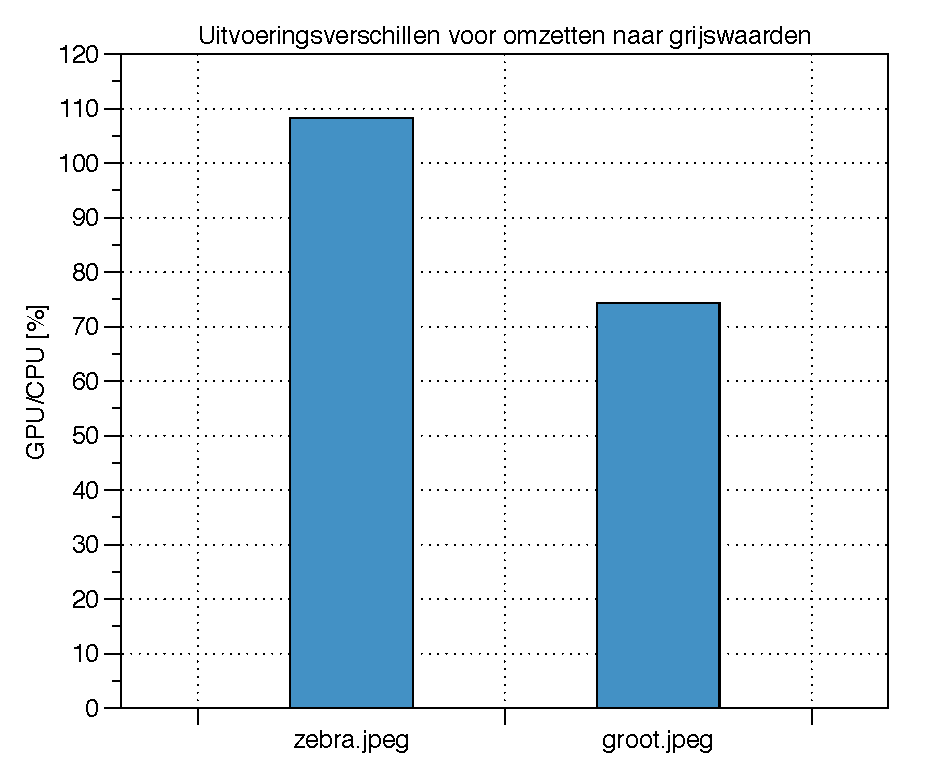
\includegraphics[width=0.5\textwidth]{grayscaling.eps}
    \caption{Executietijd $\frac{gpu}{cpu}$ \% voor grayscaling}
    \label{blocksize}
\end{figure}

\begin{figure}[H]
    \centering
    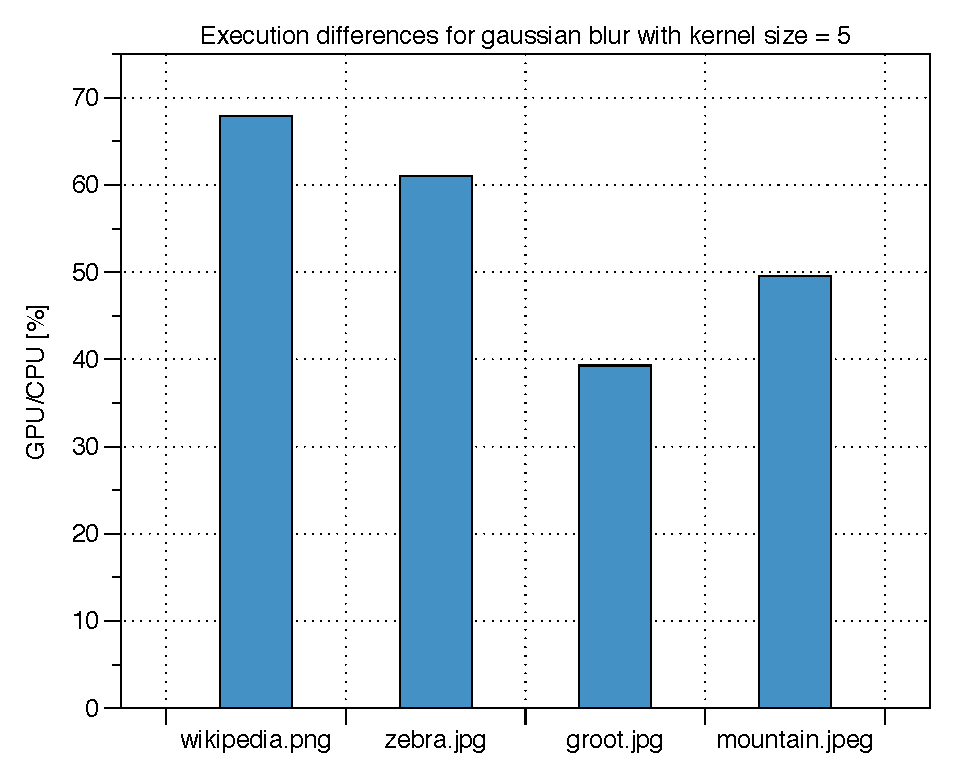
\includegraphics[width=0.5\textwidth]{gaussian_blur.eps}
    \caption{Executietijd $\frac{gpu}{cpu}$ \% voor gaussian blur (5x5)}
    \label{blocksize}
\end{figure}

\begin{figure}[H]
    \centering
    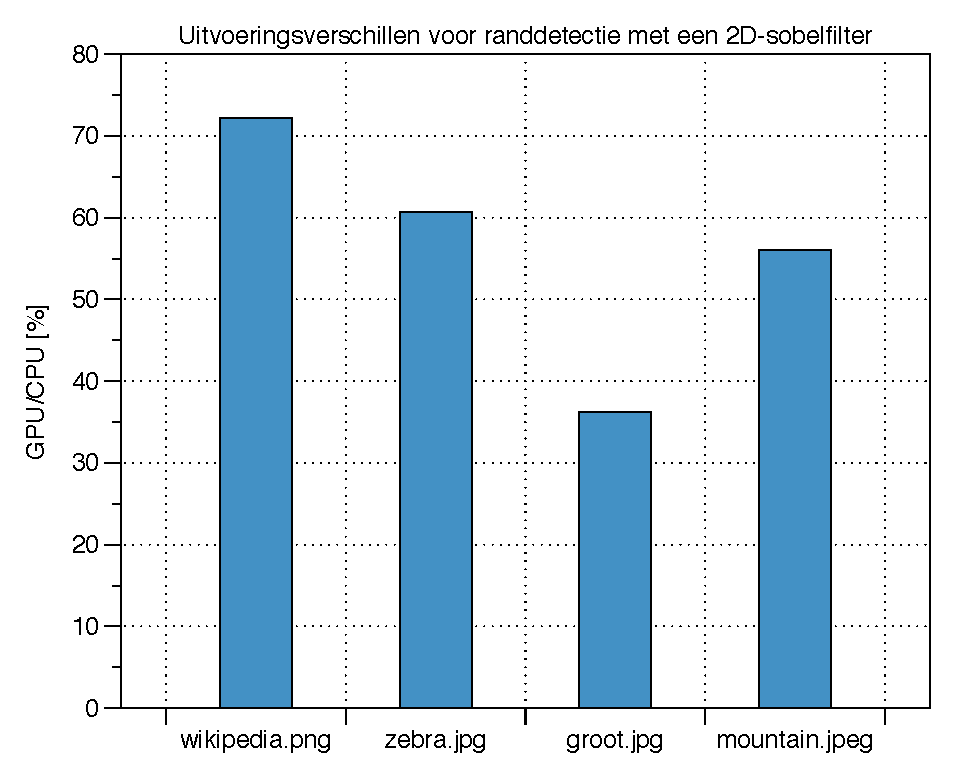
\includegraphics[width=0.5\textwidth]{edge_detection.eps}
    \caption{Executietijd $\frac{gpu}{cpu}$ \% voor edge detection (2D Sobel)}
    \label{blocksize}
\end{figure}

\section{Besluit}

\onecolumn

\appendix
\begin{figure}[H]
    \centering
    \includegraphics[width=0.75\textwidth]{test.jpg}
    \caption{Zebra.jpg}
    \label{blocksize}
\end{figure}
\begin{figure}[H]
    \centering
    \includegraphics[width=0.75\textwidth]{output_zebra.png}
    \caption{Het resultaat van zebra.jpg na de Sobel filter}
    \label{blocksize}
\end{figure}

\begin{figure}[H]
    \centering
    \includegraphics[width=0.75\textwidth]{wikipedia.PNG}
    \caption{Wikipedia.png}
    \label{blocksize}
\end{figure}
\begin{figure}[H]
    \centering
    \includegraphics[width=0.75\textwidth]{wikipedia_output.png}
    \caption{Het resultaat van Wikipedia.png na de Sobel filter}
    \label{blocksize}
\end{figure}

\begin{figure}[H]
    \centering
    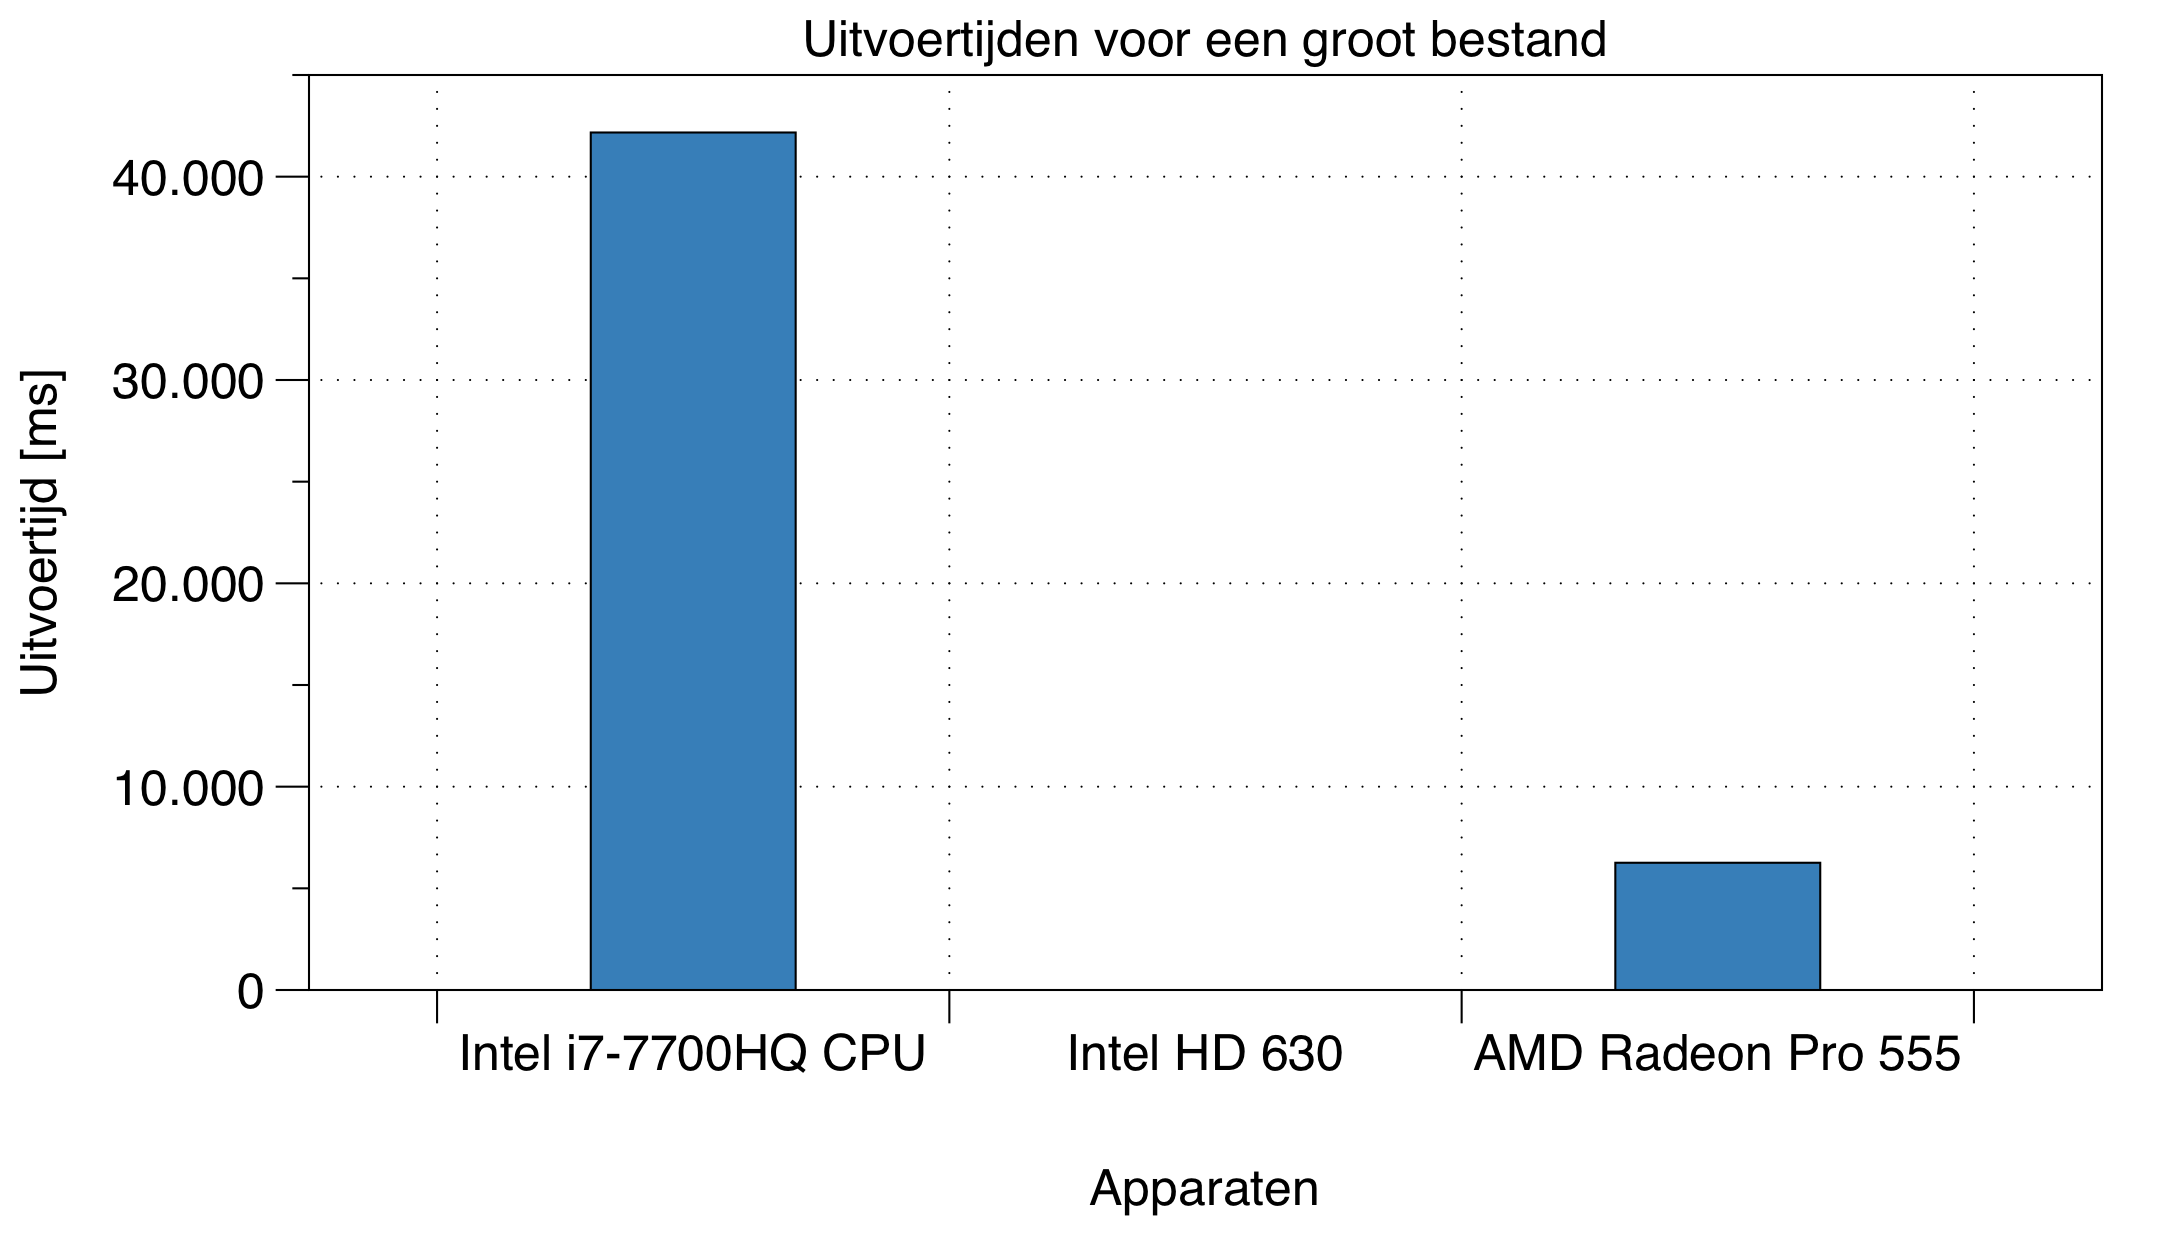
\includegraphics[width=0.75\textwidth]{groot.jpg}
    \caption{groot.jpg}
    \label{blocksize}
\end{figure}
\begin{figure}[H]
    \centering
    \includegraphics[width=0.75\textwidth]{mountain.jpeg}
    \caption{mountain.joeg}
    \label{blocksize}
\end{figure}

\newpage

\inputminted[tabsize=4,obeytabs]{c}{labo2.c}
\newpage
\inputminted[tabsize=4,obeytabs]{c}{labo2_gray.c}

% The appendix command is issued once, prior to all appendices, if any.
%\appendix
\end{document}

